% Figures for the review paper

% ===== FIGURE 1: Paradigm Shift Overview =====
\begin{figure}[t]
\centering
\resizebox{0.95\textwidth}{!}{%
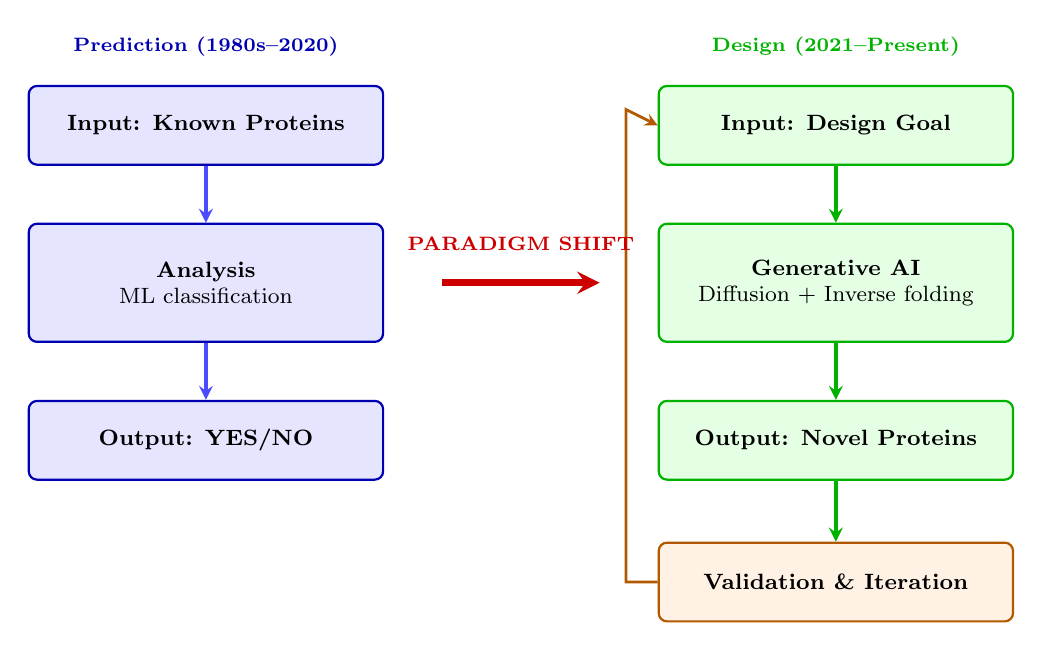
\begin{tikzpicture}[
    box/.style={rectangle, rounded corners=3pt, draw, minimum width=4.5cm, minimum height=1cm, align=center, font=\footnotesize},
    predbox/.style={box, fill=blue!10, draw=blue!70!black, line width=0.8pt},
    designbox/.style={box, fill=green!10, draw=green!70!black, line width=0.8pt},
    validatebox/.style={box, fill=orange!10, draw=orange!70!black, line width=0.8pt},
    arrow/.style={->, >=stealth, line width=1.2pt},
    predarrow/.style={arrow, blue!70},
    designarrow/.style={arrow, green!70!black}
]
% Prediction paradigm
\node[predbox] (p1) at (-4, 5) {\textbf{Input: Known Proteins}};
\node[predbox, minimum height=1.5cm] (p2) at (-4, 3) {\textbf{Analysis}\\ML classification};
\node[predbox] (p3) at (-4, 1) {\textbf{Output: YES/NO}};
\draw[predarrow] (p1) -- (p2);
\draw[predarrow] (p2) -- (p3);
\node[font=\scriptsize\bfseries, blue!70!black] at (-4, 6) {Prediction (1980s--2020)};
% Design paradigm
\node[designbox] (d1) at (4, 5) {\textbf{Input: Design Goal}};
\node[designbox, minimum height=1.5cm] (d2) at (4, 3) {\textbf{Generative AI}\\Diffusion + Inverse folding};
\node[designbox] (d3) at (4, 1) {\textbf{Output: Novel Proteins}};
\node[validatebox] (d4) at (4, -0.8) {\textbf{Validation \& Iteration}};
\draw[designarrow] (d1) -- (d2);
\draw[designarrow] (d2) -- (d3);
\draw[designarrow] (d3) -- (d4);
\draw[orange!70!black, ->, >=stealth, line width=1pt] (d4.west) -- ++(-0.4, 0) -- ++(0, 6) -- (d1.west);
\node[font=\scriptsize\bfseries, green!70!black] at (4, 6) {Design (2021--Present)};
% Center arrow
\draw[red!80!black, ->, >=stealth, line width=2.5pt] (-1, 3) -- (1, 3);
\node[font=\scriptsize\bfseries, red!80!black] at (0, 3.5) {PARADIGM SHIFT};
\end{tikzpicture}
}
\caption{The paradigm shift from prediction to design in AI-driven PPI research. \textbf{Left panel (Prediction Paradigm, 1980s--2020):} Traditional computational approaches analyze known protein sequences and structures to predict interaction likelihood (YES/NO). Blue color scheme indicates analytical methods including machine learning classification and structure comparison. \textbf{Right panel (Design Paradigm, 2021--present):} Modern AI-driven approaches generate novel protein sequences with desired interaction properties through iterative design-test cycles. Green color scheme indicates generative methods including diffusion models and inverse folding. The validation loop (orange) reflects the critical role of experimental feedback.}
\label{fig:paradigm}
\end{figure}

% ===== FIGURE 2: Technical Evolution Timeline =====
\begin{figure}[t]
\centering
\resizebox{0.95\textwidth}{!}{%
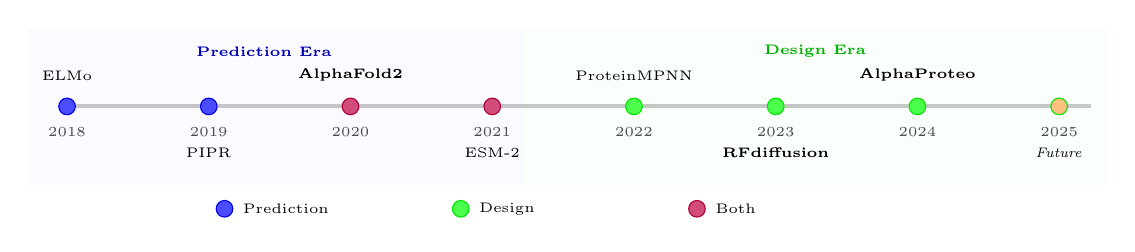
\begin{tikzpicture}[
    milestone/.style={circle, minimum size=6pt, inner sep=0pt},
    predmile/.style={milestone, fill=blue!70, draw=blue!90!black},
    designmile/.style={milestone, fill=green!70, draw=green!90!black},
    bothmile/.style={milestone, fill=purple!70, draw=purple!90!black}
]
% Timeline
\draw[line width=1.5pt, gray!60] (0, 0) -- (13, 0);
% Year markers
\foreach \x/\y in {0/2018, 1.8/2019, 3.6/2020, 5.4/2021, 7.2/2022, 9/2023, 10.8/2024, 12.6/2025} {
    \draw[gray!60] (\x, -0.1) -- (\x, 0.1);
    \node[font=\tiny, below] at (\x, -0.15) {\y};
}
% Phase backgrounds
\fill[blue!5, opacity=0.3] (-0.5, -1) rectangle (5.8, 1);
\fill[green!5, opacity=0.3] (5.8, -1) rectangle (13.2, 1);
\node[font=\tiny\bfseries, blue!70!black] at (2.5, 0.7) {Prediction Era};
\node[font=\tiny\bfseries, green!70!black] at (9.5, 0.7) {Design Era};
% Milestones
\node[predmile] at (0, 0) {};
\node[font=\tiny, above, align=center] at (0, 0.2) {ELMo};
\node[predmile] at (1.8, 0) {};
\node[font=\tiny, below, align=center] at (1.8, -0.4) {PIPR};
\node[bothmile] at (3.6, 0) {};
\node[font=\tiny, above, align=center] at (3.6, 0.2) {\textbf{AlphaFold2}};
\node[bothmile] at (5.4, 0) {};
\node[font=\tiny, below, align=center] at (5.4, -0.4) {ESM-2};
\node[designmile] at (7.2, 0) {};
\node[font=\tiny, above, align=center] at (7.2, 0.2) {ProteinMPNN};
\node[designmile] at (9, 0) {};
\node[font=\tiny, below, align=center] at (9, -0.4) {\textbf{RFdiffusion}};
\node[designmile] at (10.8, 0) {};
\node[font=\tiny, above, align=center] at (10.8, 0.2) {\textbf{AlphaProteo}};
\node[designmile, fill=orange!50] at (12.6, 0) {};
\node[font=\tiny, below, align=center] at (12.6, -0.4) {\textit{Future}};
% Legend
\node[predmile, label=right:{\tiny Prediction}] at (2, -1.3) {};
\node[designmile, label=right:{\tiny Design}] at (5, -1.3) {};
\node[bothmile, label=right:{\tiny Both}] at (8, -1.3) {};
\end{tikzpicture}
}
\caption{Timeline of major technical breakthroughs in AI-driven protein research (2018--2025). The paradigm shift from prediction to design occurred around 2021--2022, marked by the emergence of generative methods. \textbf{Milestones in bold} (AlphaFold2, RFdiffusion, AlphaProteo) represent transformative advances with extensive experimental validation. \textbf{Color coding:} Blue = prediction-focused; green = design-focused; purple = spanning both paradigms. Shaded regions delineate the Prediction Era (2018--2021) from the Design Era (2022--present).}
\label{fig:timeline}
\end{figure}
